\documentclass[10pt,a4paper]{article}
\usepackage[utf8]{inputenc}
\usepackage[german]{babel}
\usepackage[T1]{fontenc}
\usepackage{amsmath}
\usepackage{amsfonts}
\usepackage{amssymb}
\usepackage{hyperref}
\usepackage{graphicx}
\usepackage[usenames,dvipsnames]{xcolor}
\usepackage{tikz}
\usepackage{listingsutf8}
\usepackage{color}
\usetikzlibrary{patterns}
\usepackage{units}
\usepackage{nameref}
\usepackage{caption}
\usepackage[left=2cm,right=2cm,top=2cm,bottom=2cm]{geometry}

\title{Arduino-Grundkurs}
\author{Julian Heinzel}

% Configuring listings.
\lstset
{
	language=c++,
	keywordstyle=\color{NavyBlue},
	numbers=left,
	numberstyle=\small,
	stringstyle=\color{OliveGreen},
	commentstyle=\color{ForestGreen},
	showstringspaces=false
}
\renewcommand{\lstlistingname}{Codeblock}
\DeclareCaptionFont{white}{\color{white}}
\DeclareCaptionFormat{listing}{\colorbox[cmyk]{0.43, 0.35, 0.35,0.01}{\parbox{.98\textwidth}{\hspace{15pt}#1#2#3}}}
\captionsetup[lstlisting]{format=listing,labelfont=white,textfont=white}
% Changing font so sans serif.
\renewcommand{\familydefault}{\sfdefault}


\begin{document}
\begin{center}
	\makeatletter
	{\LARGE\textbf{\@title}}\\\bigskip
	{\Large\@author}\\\medskip
	{\large\@date}\\
	\makeatother
	\vspace{0.3cm}
	\begin{tikzpicture}
		\draw (0,0) -- (5,0);
	\end{tikzpicture}
	\\\medskip
	Lizensiert als Creative Commons Attribution 4.0\\
	https://creativecommons.org/licenses/by/4.0/legalcode
	\\\medskip
	
\includegraphics[width=0.75cm]{CC.png}
	
\includegraphics[width=0.75cm]{BY.png}
\end{center}
\vspace{0.3cm}
\tableofcontents
\vspace{1cm}


\section{Einleitung}
Arduino ist eine sogenannte "`Physical computing"'-Plattform, die auf einem einfachen Mikrocontroller und einer dazugehörigen \emph{IDE} (Integrated Development Environment) basiert. Damit können leicht Projekte umgesetzt werden, die mit ihrer Umwelt interagieren, Messungen vornehmen und Geräte steuern. Die folgenden Aufgaben sollen eine Einführung in die Programmierung dieser Plattform darstellen und beziehen sich auf den \emph{Arduino Uno}.
\bigskip

Als Programmiersprache kommt C/C++ zum Einsatz, welches um die Arduino-Bibliothek erweitert wurde. Alle darin enthaltenen Befehle können auf der Homepage arduino.cc unter Reference eingesehen werden. Auf der Website befinden sich außerdem zahlreiche Beispiele und Tutorials.
\bigskip

Ein leeres Arduinoprojekt enthält mindestens zwei Funktionen:
\begin{lstlisting}
void setup()
{
}

void loop()
{
}
\end{lstlisting}

Diese werden von der Arduino-Bibliothek deklariert und müssen stets vorhanden sein. \emph{setup} wird dabei einmal zu Anfang ausgeführt und sollte Anweisungen enthalten, die den Arduino wie benötigt konfigurieren.
\emph{loop} wird daraufhin unablässig wiederholt.


\clearpage
\section{Digitaler Output}
% Reconfiguring listing style
\lstset
{
	numbers=none,
	backgroundcolor=\color[gray]{0.85}
}

Der Arduino Uno besitzt 13 digitale Ein- bzw. Ausgänge. Digital heißt, dass diese nur zwischen zwei Zuständen unterscheiden können: \emph{HIGH} oder \emph{LOW}, bzw. null oder fünf Volt. Damit kann zum Beispiel eine LED ein- und ausgeschaltet werden.

In den Arduino ist auf Port D13 bereits eine LED eingebaut, es kann aber genauso eine externe LED angeschlossen werden. Dabei muss jedoch unbedingt ein Vorwiderstand angeschlossen werden, um den Strom durch die LED auf circa \unit[20]{mA} zu begrenzen: Ansonsten löst diese oder der Arduino sich in magischen Rauch auf.
\bigskip

Zuerst muss in der Setupfunktion definiert werden, dass der betreffende Port als Output verwendet werden soll, also dass damit ein anderes Gerät mit Strom und Spannung versorgt werden soll. Dazu existiert die Funktion
\begin{lstlisting}
	void pinMode(int pin, int mode)
\end{lstlisting}
\bigskip

Danach kann in der loop mit \emph{digitalWrite} der verwendete Pin auf HIGH gesetzt werden.
\begin{lstlisting}
	void digitalWrite(int pin, int mode)
\end{lstlisting}
\bigskip

Die Ausführung des Programms lässt sich mit mit zwei Funktionen unterbrechen:
\begin{lstlisting}
	void delay(int milliseconds)
	void delayMicroseconds(int microseconds)
\end{lstlisting}
\bigskip

Weitere Informationen über die genannten Funktionen sind auf der offiziellen Webseite arduino.cc zu finden.
\begin{itemize}
	\item Schreibe ein Programm, das eine LED für einige Sekunden einschaltet und danach einige Sekunden ausschaltet.
\end{itemize}


\section{Digitaler Input}
\label{DigitalInput}
Die digitalen Ports können auch als Input definiert werden. Dabei gelten Spannungen über \unit[3.3]{V} als HIGH, Spannungen darunter als LOW. Analog gibt es eine Funktion, die den Signalpegel für den gewünschten Pin überprüft:
\begin{lstlisting}
	int digitalRead(int pin)
\end{lstlisting}
\bigskip

Dabei wird man anfangs versucht sein, die Schaltung nach Abbildung \ref{NoPulldown} wie folgt aufzubauen:

\begin{figure}[htbp!]
\begin{minipage}{0.5\textwidth}
	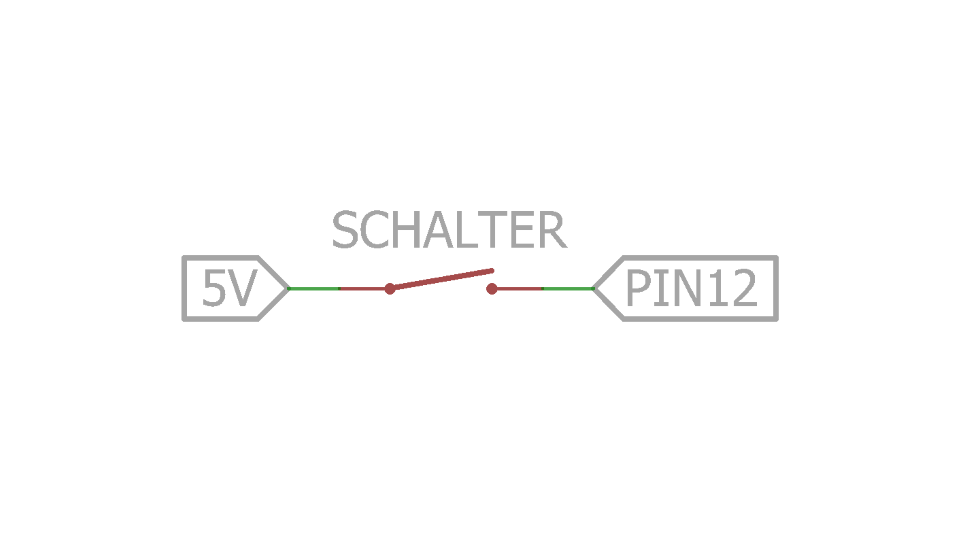
\includegraphics[width=\textwidth]{NoPulldown.png}
	\caption{Schaltung ohne Pulldown-Widerstand}	
	\label{NoPulldown}
\end{minipage}
\begin{minipage}{0.5\textwidth}
	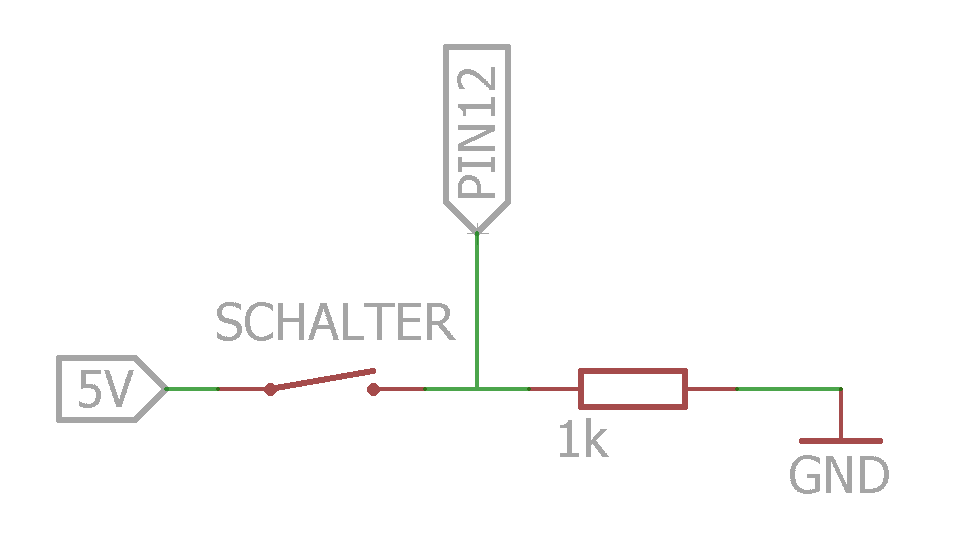
\includegraphics[width=\textwidth]{Pulldown.png}
	\caption{Schaltung mit Pulldown-Widerstand}
	\label{Pulldown}
\end{minipage}
\end{figure}

Solange der Schalter geschlossen ist, wird man auf Pin 12 HIGH messen. Wird dieser jedoch geöffnet, so liegt der Pin nicht mehr auf HIGH - aber auch nicht auf LOW. Das Potential ist an dieser Stelle undefiniert, der Eingang "`floatet"', nimmt störende Felder aus seiner Umgebung auf und misst so eine mehr oder weniger zufällige Spannung.
Abhilfe schafft Schaltung \ref{Pulldown}. Ist der Schalter geschlossen, so fällt die gesamte Spannung an dem \emph{Pulldown-Widerstand} ab, am Eingang liegen wie zuvor \unit[5]{V}. Im geöffneten Zustand jedoch wird der Eingang über den Widerstand auf Massepotential gezogen, am Eingang wird LOW gemessen.
Analog lassen sich auch \emph{Pullup-Widerstände} einsetzen.

\begin{itemize}
	\item Schreibe ein Programm, welches in jedem Durchgang der Hauptschleife überprüft, ob ein Schalter gedrückt ist und dementsprechend eine LED an- oder ausschaltet.
\end{itemize}


\clearpage
\section{Funktionen}
\begin{itemize}
	\item Schreibe eine Funktion vom Datentyp \emph{void}, welche einen Ton zufälliger Höhe auf einem Lautsprecher abspielt. Suche dafür in der Referenz auf arduino.cc geeignete Funktionen, um einen Ton zu erzeugen.
\end{itemize}


\section{Analoger Input}
Der Mikrocontroller kann nicht nur zwischen HIGH und LOW unterscheiden, sondern über die analogen Inputs A1 bis A6 auch die genaue Größe einer Spannung ermitteln. Die Spannung zwischen \unit[0]{V} und \unit[5]{V} wird als 10-Bit-Ganzzahl dargestellt, also als Wert zwischen 0 und 1023.

\begin{itemize}
	\item Schließe ein Potentiometer zwischen \unit[0]{V} und \unit[5]{V} an und erstelle so eine variable Spannungsquelle.
	\item Schließe fünf LEDs an, von denen je nach Spannung jeweils eine leuchten soll. Vorwiderstand nicht vergessen!
\end{itemize}


\section{Serielle Kommunikation}
\subsection{Daten senden}
Über die serielle Schnittstelle kann der Mikrocontroller mit dem angeschlossenen Computer oder anderen Geräten kommunizieren. Dazu muss in der Setup-Funktion die Kommunikation mit einer bestimmten Baudrate (Symbole pro Sekunde) gestartet werden. Die am PC ankommenden Daten können dann im "`Serial Monitor"' der Arduino-Umgebung eingesehen werden. Folgende Funktionen sind unter anderem wichtig:

% Reconfiguring listing style
\lstset
{
	numbers=none,
	backgroundcolor=\color[gray]{0.85}
}
\begin{lstlisting}
	void Serial.begin(speed)
\end{lstlisting}
und
\begin{lstlisting}
	long Serial.println(value)
\end{lstlisting}

\begin{itemize}
	\item Wandle das Programm aus der letzten Aufgabe so ab, dass die aktuell gemessene Spannung auf dem Computer angezeigt wird.
	\item Falls du nicht weiter kommst, hilft dir die Website arduino.cc.
\end{itemize}

\subsection{Daten empfangen}
Es können nicht nur Daten gesendet werden - der Arduino kann auch Daten vom Computer empfangen. Dazu können die folgenden Funktionen verwendet werden:

\begin{lstlisting}
	int Serial.available(void)
\end{lstlisting}
\begin{lstlisting}
	int Serial.read(void)
\end{lstlisting}

\begin{itemize}
	\item Der Arduino soll nun den seriellen Port auf ankommende Befehle überprüfen. Wird eine Zahl zwischen eins und fünf empfangen, soll die Messung des Potentiometers ignoriert und die entsprechende LED eingeschaltet werden. Wird das Potentiometer verstellt, so soll erneut die Spannungsmessung bestimmend für die LEDs sein.
\end{itemize}


\clearpage
\section{PWM-Output}
Im Gegensatz zu anderen Mikrocontrollern besitzt der Arduino Uno keine Digital-Analog-Wandler (DAC), um Spannungen zwischen null und fünf Volt zu erzeugen. In vielen Fällen kommt als Ersatz jedoch die Verwendung eines \emph{PWM-Signals} in Frage. PWM steht für \emph{Pulse Width Modulation} - dabei wird ein Rechtecksignal fester Frequenz erzeugt, jedoch die Zeit variiert, die das Signal auf HIGH-Pegel liegt:

\begin{figure}[htbp!]
\begin{minipage}{0.5\textwidth}
	\begin{tikzpicture}
		% Horizontal axis.
		\draw[->] (0,0) -- (6.5,0) node[anchor=north] {Periode};
		\draw	(0,0) node[anchor=north] {0}
				(2,0) node[anchor=north] {1}
				(4,0) node[anchor=north] {2};
		
		% Vertical axis.
		\draw[->] (0,0) -- (0,4) node[anchor=east] {$U$};
		\draw	(0,0) node[anchor=east] {0V}
				(0,3) node[anchor=east] {5V};
		
		% PWM signal.						
		\draw[pattern=north west lines, pattern color=CornflowerBlue]
			(0,0) rectangle (0.5,3)				
			(2,0) rectangle (2.5,3)
			(4,0) rectangle (4.5,3);
			
		\draw[thick]	(0,3) -- (0.5,3) -- (0.5,0) -- (2,0) -- (2,3)
						(2,3) -- (2.5,3) -- (2.5,0) -- (4,0) -- (4,3)
						(4,3) -- (4.5,3) -- (4.5,0);

	\end{tikzpicture}
	\caption{PWM-Signal mit 25\% Pulsweite}
\end{minipage}
\begin{minipage}{0.5\textwidth}
	\begin{tikzpicture}
		% Horizontal axis.
		\draw[->] (0,0) -- (6.5,0) node[anchor=north] {Periode};
		\draw	(0,0) node[anchor=north] {0}
				(2,0) node[anchor=north] {1}
				(4,0) node[anchor=north] {2};
		
		% Vertical axis.
		\draw[->] (0,0) -- (0,4) node[anchor=east] {$U$};
		\draw	(0,0) node[anchor=east] {0V}
				(0,3) node[anchor=east] {5V};
		
		% PWM signal.					
		\draw[pattern=north west lines, pattern color=CornflowerBlue]
			(0,0) rectangle (1.5,3)				
			(2,0) rectangle (3.5,3)
			(4,0) rectangle (5.5,3);
			
		\draw[thick]	(0,3) -- (1.5,3) -- (1.5,0) -- (2,0) -- (2,3)
						(2,3) -- (3.5,3) -- (3.5,0) -- (4,0) -- (4,3)
						(4,3) -- (5.5,3) -- (5.5,0);
	\end{tikzpicture}
	\caption{PWM-Signal mit 75\% Pulsweite}
\end{minipage}
\end{figure}

Das Verhältnis von Ein- und Ausschaltdauer der Impulse nennt man \emph{Pulsweite} oder \emph{Duty Cycle}. Über die Modulation dieser Pulsweite lässt sich zum Beispiel die Helligkeit einer LED oder die Geschwindigkeit eines Motors regeln: Da das menschliche Auge bzw. die Mechanik zu träge ist, um die einzelnen Pulse aufzulösen und voneinander zu trennen, ergibt sich effektiv eine mittlere Spannung zwischen null und fünf Volt.

Alternativ ließe sich das Rechtecksignal mit einem großen Kondensator oder einer Induktivität glätten, die die Spannung puffern und die dahinter liegende Schaltung versorgen, solange das PWM-Signal LOW ist.

\bigskip
Servomotoren interpretieren das PWM-Signal im Gegensatz zu normalen Gleichstrommotoren als Position und drehen sich je nach Pulsweite in die entsprechende Position.

Nicht alle digitalen Pins eines Mikrocontrollers können ein PWM-Signal erzeugen. Bei einem Arduino Uno sind das zum Beispiel nur die Pins 3, 5, 6, 9, 10 und 11, das lässt sich auf der Website arduino.cc auh für andere Arduinomodelle nachschlagen. Diese Pins können verwendet werden, um die Funktion

\begin{lstlisting}
	void analogWrite(pin, value)
\end{lstlisting}

aufzurufen. \textit{value} ist dabei die Pulsweite, angegeben als Zahl zwischen 0 (immer aus) und 255 (immer an). Um \textit{analogWrite} verwenden zu können, muss der Pin übrigens nicht mit \textit{pinMode} als Ausgang definiert werden.


\begin{itemize}
	\item Baue eine Schaltung aus einer LED mit Vorwiderstand an einem PWM-fähigen Pin.
	\item Schreibe eine Funktion, die als Parameter einen Pin und die gewünschte Helligkeit annimmt und die LED via \textit{analogWrite} anschaltet.
\end{itemize}


\section{Interrupts}
% Reconfiguring listing style
\lstset
{
	numbers=none,
	backgroundcolor=\color[gray]{0.85}
}

Die dimmbare LED aus der vorherigen Aufgabe soll nun via Knopfdruck durch einen \emph{Interrupt} gesteuert werden. Interrupts sind hardwaremäßig in den Mikrocontroller eingebaut und können auf äußere Umstände reagieren. Sie können den aktuell ausgeführten Code unterbrechen ("`Interrupt"') und anstatt dessen "`zwischendurch"' eine andere Funktion auslösen. Welche Funktion das ist und unter welcher Bedingung der Interrupt ausgelöst wird, kann mit der Methode

\begin{lstlisting}
	void attachInterrupt(int interrupt, void (*function) (void), int mode)
\end{lstlisting}

festgelegt werden. Mit ihr kann eine Funktion sozusagen "`An einen Interrupt angeheftet"' werden. \emph{mode} kann dabei \emph{RISING}, \emph{FALLING}, \emph{CHANGE} oder \emph{LOW} sein und bestimmt, wann der Interrupt ausgelöst wird. RISING bedeutet in diesem Fall zum Beispiel, dass der Interrupt immer dann ausgelöst wird, wenn die Spannung am dazugehörigen Pin von LOW auf HIGH springt.

Von diesen Interruptpins verfügt der Arduino Uno über zwei Stück, welche von null an aufwärts nummeriert werden und den digitalen Pins zwei und drei entsprechen. Um diese beiden Nummerierungsarten verständlich und unabhängig vom verwendeten Microcontroller ineinander zu überführen, existiert die Funktion

\begin{lstlisting}
	int digitalPinToInterrupt(int pin)
\end{lstlisting}
Auf einem Arduino Uno wird durch diese Funktion also zum Beispiel zwei zu null und drei zu eins.
\bigskip


\clearpage
% Reconfiguring listing style
\lstset
{
	numbers=left,
	backgroundcolor=\color{white}
}
\begin{lstlisting}[caption=Ausschnitt aus dem Programmcode einer Messbox des Windkraftwerks, label=Drehzahlmessung] 
volatile int rounds = 0;
const int rpmPin = 3;

void setup()
{
  pinMode(rpmPin, INPUT_PULLUP);
  attachInterrupt(digitalPinToInterrupt(rpmPin), count, FALLING);
}

void loop() { }

void count()
{
  rounds++;
}
\end{lstlisting}
\vspace{0.5cm}

Interrupts werden zum Beispiel bei der Drehzahlmessung des drachenbasierten fliegenden Windkraftwerks verwendet, das in Jahren 2014 bis 2016 am Aerospace Lab Herrenberg entwickelt wurde. Ein Auszug der dort verwendeten Software ist in Codeblock \ref{Drehzahlmessung} dargestellt. In Zeile sechs wird der interne Pullup-Widerstand von Pin drei aktiviert, der Pin liegt also im Normalfall über $\unit[20]{k\Omega}$ auf \unit[5]{V} und ist mit der Lichtschranke verbunden. Wird die Lichtschranke jedoch nicht mehr blockiert, schaltet der darin befindliche Fototransistor durch und zieht Pin drei auf Nullpotential.

Da die Spannung von \unit[5]{V} auf \unit[0]{V} \emph{abfällt} (FALLING), wird die Funktion \emph{count} ausgelöst und die Variable \emph{rounds} inkrementiert - wie in Zeile sieben definiert.

\begin{itemize}
	\item Ergänze die Schaltung aus der vorherigen Aufgabe um einen Schalter an einem der Interruptpins. Der Schalter kann den Pin bei Aktivierung zum Beispiel mit \unit[5]{V} verbinden. Vergiss in diesem Fall nicht einen Pull-Down-Widerstand wie in Aufgabe \ref{DigitalInput} (\nameref{DigitalInput}) zu verbauen, sodass bei deaktiviertem Schalter auch tatsächlich \unit[0]{V} an dem Interrupt anliegen.
	\item Schreibe eine Funktion \textit{step}, die die LED mit jedem Knopfdruck etwas heller stellt. Du kannst dabei auf die Funktionen aus der vorherigen Aufgabe zugreifen.
	\item Wenn die LED mit maximaler Helligkeit leuchtet, soll der nächste Aufruf der Funktion \textit{step} sie wieder ausschalten.
\end{itemize}



%
% Sources
%
\bigskip
\section*{Quellen}

\begin{itemize}
	\item http://www.arduino.cc/en/Reference/attachInterrupt, 9. April 2016
	\item http://timogruss.de/2013/07/die-timer-des-atmega128-pwm-modus-1, 9. April 2016
	\item https://www.arduino.cc/en/Reference/AnalogWrite, 25. November 2016
\end{itemize}

\end{document}